\documentclass[14pt, a4paper]{extarticle}
\usepackage[utf8x]{inputenc}
\usepackage[russian]{babel}
\usepackage{graphicx}
\usepackage{float}
\usepackage[outdir=./]{epstopdf}
\usepackage{booktabs}
\usepackage{tocvsec2}
\usepackage{amsfonts}
\usepackage{amsmath}
\usepackage[left=2cm,right=2cm,bottom=3cm,top=2cm]{geometry}

\graphicspath{ {./images/} }

\linespread{1.25}

\begin{document}

\thispagestyle{empty}

\begin{center}
\ \vspace{-4cm}

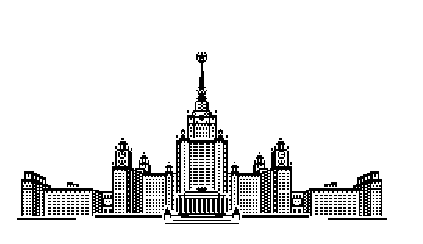
\includegraphics[width=0.5\textwidth]{msu}\\
{Московский государственный университет имени М.В. Ломоносова}\\
Факультет вычислительной математики и кибернетики\\
Кафедра автоматизации систем вычислительных комплексов

\vspace{5cm}

{\Large Долганов Станислав Викторович}

\vspace{1cm}

{\Large\bfseries
Метод поиска несоответствий границ объектов между результатом 2D-3D конвертации 
и используемыми картами глубины\\}

\vspace{1cm}

{\large ВЫПУСКНАЯ КВАЛИФИКАЦИОННАЯ  РАБОТА}
\end{center}

\vfill

\begin{flushright}
  \textbf{Научный руководитель:}\\
  к.ф-м.н.\\
  Д.С. Ватолин
\end{flushright}

\vfill

\begin{center}
Москва, 2016
\end{center}

\enlargethispage{4\baselineskip}

\newpage
% Аннотация (не более полстраницы) содержит формулировку задачи и основных результатов.

\textbf{Метод поиска несоответствий границ объектов между результатом 2D-3D конвертации 
и используемыми картами глубины}

\vspace{0.5cm}
Станислав Долганов
\vspace{0.5cm}

При создании полнометражных и любительских трехмерных фильмов с помощью 
конвертации отснятого в 2D материала достаточно часто возникают дефекты, 
связанные с качеством используемых карт глубины. Такого рода артифакты, 
даже если они находятся вне салиентных регионов,  могут заметно ухудшить 
восприятие смотрящего, и более того~---~вызвать головную боль. В дипломной
работе предлагается метод поиска объектов переднего плана, границы которых 
в стерео сцене не совпадают с действительностью, то есть объектов слитых 
с фоном. Предлагаемый метод извлекает информацию о движении в сцене и 
находит несоответствия конвертации между извлеченным движением и глубиной сцены.
Метод был применен на 39 полнометражных фильмах, что позволило найти 125 сцен с заметными несоответствиями границ объектов между картой движения и картой глубины, 
использованной при конвертации.

\vspace{2cm}

\textbf{Object boundaries inconsistencies detection method 
for 2D-3D (Two-Dimensional-Three-Dimensional)
conversion results and depth maps}

\vspace{0.5cm}
Stanislav Dolganov
\vspace{0.5cm}

The creation of S3D movies by converting 2D captured footage
often introduces depth-map inaccuracies. Such artifacts can
significantly degrade the viewing experience even if they occur
only in unsalient background objects.
In this paper we propose a method for detecting foreground
objects that are stuck to the background. Our method extracts
information about motion in the scene and detects conversionrelated
discrepancies between motion strength and depth. We
demonstrate the performance of the method by applying it
to 39 full-length converted 3D movies and by providing the
results of our analysis as well as examples of detected problem
shots.

\newpage
\addcontentsline{toc}{section}{Содержание}
\tableofcontents

\newpage
\section{Введение}
% Введение должно описывать предметную область, к которой относится задача, 
% решаемая в дипломной работе, содержать неформальное ее описание.

\subsection{Стереоскопическое видео и конвертация}

В наше время практически в каждом кинотеатре мира обязательно найдется сеанс в 3D. 
Такой интерес порождает повышенный спрос на стерео контент, однако развитие 
современных технологий производства 3D фильмов не способно в полной мере ему отвечать. 
Стандартный процесс создания контента происходит тремя возможными путями: 
\begin{itemize}
	\item съемка с помощью дорогостоящих стереоскопических систем камер,
	\item конвертация заранее отснятого двухмерного материала,
	\item использование компьютерной графики.
\end{itemize}
Последний подход относится к специфичной области мультипликационных фильмов, 
а также позволяет создавать различные спецэффекты на этапе постобработки. 
Съемка видео с помощью стерео камер требует постоянной каллибровки цветовых и 
геометрических парметров камер системы, что является не тривиальным процессом и 
потому зачастую приводит к некачественному контенту.  Учитывая последние разработки 
в области стерео конвертации~\cite{ndjiki2011depth,tolstaya2015depth}, которые 
заметно улучшили визуальное качество результата, а также сравнительно меньшие 
затраты на производство, легко заметить, что многие киностудии предпочитают 
конвертацию остальным подходам. В данном факте можно убедиться, если посмотреть 
на ежегодные соотношения конвертированных и отснятых фильмов за последние 60 лет~\cite{realorfake}.

\subsection{Проблемы конвертации} 

Хотя существующие программные инструменты на порядок облегчают различные 
этапы конвертации видео, сам процесс остается достаточно трудоемким и 
далеким от автоматизации. Майк Сеймор в своем обзоре~\cite{seymour2012art} 
описывает основные проблемы генерации стереовидео по исходному 2D материалу:
\begin{itemize}
	\item Эффект параллакса --- означает, что для генерации второго ракурса 
	необходимо заполнять области сцены, которые не видны на исходном ракурсе. 
	Основная проблема заключается в выборе материала для заполнения открывающихся 
	областей, который не вызывал бы дискомфорта при просмотре и был бы стабильным во времени.
	\item Эффект кулисности --- означает, что для объектов переднего плана необходимо 
	сгенерировать различную глубину для различных частей объекта, что позволит сделать 
	объект рельефным, иначе при просмотре сцены объект будет казаться плоским, 
	что противоречит реальной жизни.
	\item Эффект отжимающего действия рамки --- возникает, когда объекты с отрицательным 
	параллаксом, то есть такие объекты, которые при просмотре кажутся ближе к зрителю, 
	чем плоскость экрана, пересекают рамку экрана. Появлятся невозможная в реальной 
	жизни ситуация, когда часть объекта находится перед нами, а оставшаяся часть скрыта 
	более удаленной рамкой. Наиболее точно такую ситуацию можно объяснить следующим 
	образом --- представить, что объект находится перед окном и начинает двигаться 
	от центра окна к его краю, затем часть объект пересекающая границу окна пропадает.
	\item Агрессивная величина параллакса --- может проявляться различными путями. 
	Первый возможный вариант---это большие значения как положительного, так и 
	отрицательного параллакса в сцене, что влечет за собой большой разброс объектов 
	в сцене, тяжело переносится зрителем и может стать причиной головной боли. 
	Второй вариант заключается в значительном изменении отрицательного и положительного 
	параллаксов между двумя соседними сцены. Такая ситуация требует от зрителя 
	адаптироваться к каждой сцене, что также может сильно утомлять.
	\item Некачественная карта глубины. Общее качество карты глубины, которая является 
	необходимой частью процесса конвертации, прямым образом влияет на результат, 
	поэтому очень важно контролировать соответствие карты действительности, 
	что касается как верного выбора расположения объектов по глубине в сцене, 
	так и точных границ объектов.
\end{itemize}

Эффект кулисности и остальные дефекты карт глубины, которые возникают в процессе 
конвертации из 2D в 3D часто ухудшают общее восприятие зрителя от просмотра фильма. 
Наиболее значимые проблемы создают объекты, находящиеся в салиентных областях 
сцены, границы по движению которых не совпадают с границами по глубине, то есть 
таких объектов, которые движутся про пространству сцены не равномерно или деформируются, 
что не возможно в реальной жизни. Исследования в этой области~\cite{jung2012visual,li2014visual} подтверждают ухудшение состояния группы людей, которые смотрят такого рода стереовидео.

\subsection{Полуавтоматический контроль качества конвертации}

\begin{figure}[!h]
	\begin{minipage}[b]{1.0\linewidth}
		\centering
		\centerline{ 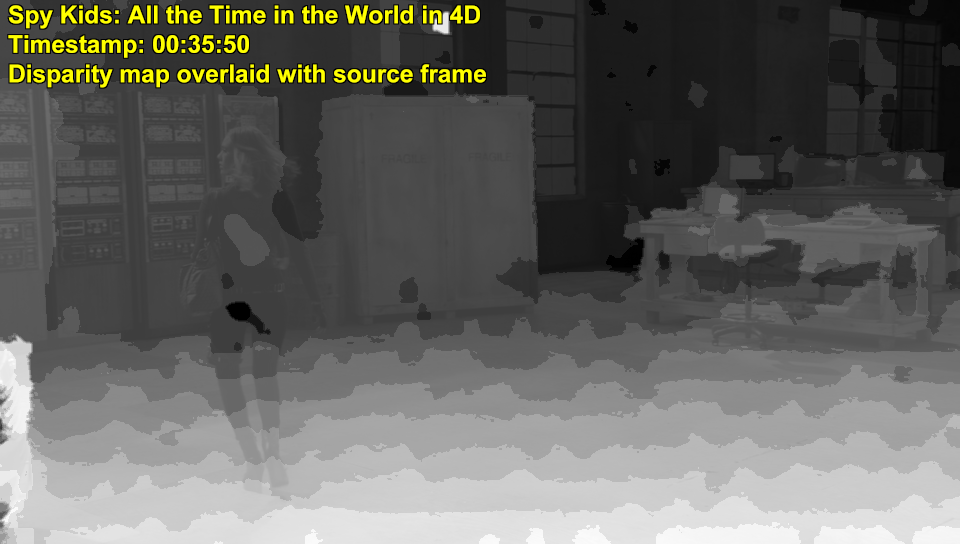
\includegraphics[width=0.7\textwidth]{example_depth} }
	\end{minipage}
	\begin{minipage}[b]{1.0\linewidth}
		\centering
		\centerline{ 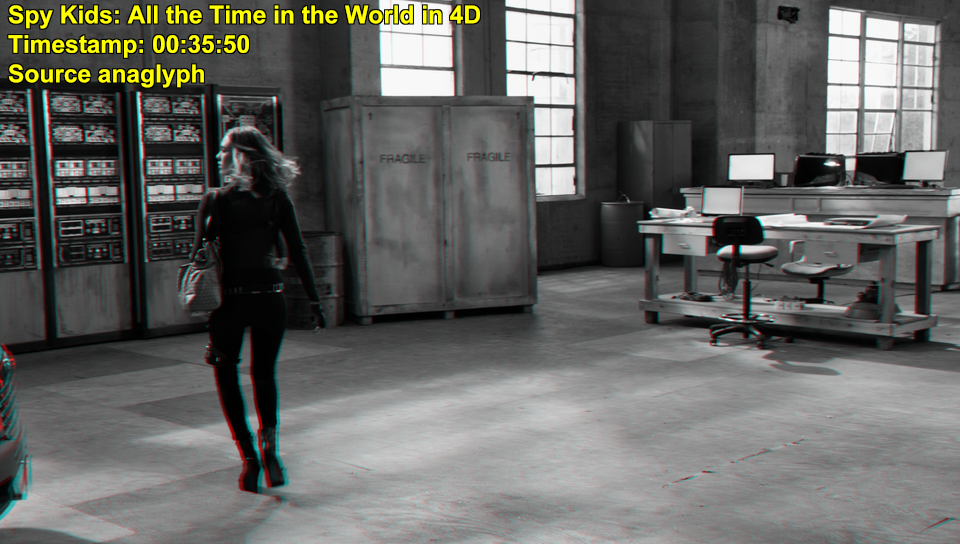
\includegraphics[width=0.7\textwidth]{example_anaglyph} }
	\end{minipage}
    \caption{Пример найденной с помощью предлагаемого метода сцены, содержащей дефект: объект переднего плана оказался слитым с фоном. Создатели фильма забыли нарисовать тело актрисы на карте глубины, поэтому сцена демонстрирует невозможную ситуацию и может вызвать визуальный дискомфорт. На верхнем изображении показана карта диспаратности поверх исходного ракурса, на нижнем --- исходная сцена в анаглифе. }
	\label{fig:example}
\end{figure}


Основной целью данной дипломной работы является создание программного инструмента, 
который позволит автоматически оценить качество используемых карт глубины,
что в свою очередь позволит киностудиям создавать более качественный контент. 
Частой практикой киностудии является разделение фильма на крупные части, которые 
затем отправляются на конвертацию в специализированные компании. Такой подход 
ухудшает качество, так как компании не знают о результатах работы друг друга. 
Основной выигрыш для киностудии---это уменьшение времени, которое понадобиться 
для конвертации, однако из-за сжатых сроков, а так же ручного тестирования 
качества результата, часто возникают такие сцены как на Рис.~\ref{fig:example}. 
Предлагаемый программный инструмент позволит проводить проверку в полуавтоматическом 
режиме, что несомненно повысит как качество, так и время производства.
В качестве входных данных предлагаемому алгоритму требуются стерео видеопоследовательность 
и опционально карты глубины, используемые во время конвертации в 3D формат данной видеопоследовательности. В случаях, когда информация об используемых картах 
глубины недоступна, метод оценивает карту диспаратности с помощью~\cite{simonyan2008fast,zhang2014100+}. Он находит дефекты сравнивая 
для каждого отдельного кадра границы карты глубины/диспаратности с границами карты 
амплитуды движения. Такой подход позволяет находить движущиеся объекты, которые 
частично или полностью отсутствуют на оцениваемой карте глубины. Так как не существует 
общепринятого быстрого и качественного алгоритма оценки векторов движения, было принято 
решение использовать в качестве такого алгоритма~\cite{simonyan2008fast}, который 
применяется к последовательности левых ракурсов. Затем полученная последовательность 
оценненых карт амплитуды движения итеративно улучшается с помощью временных и 
пространнственных фильтраций~\cite{fecker2007time,matyunin2011temporal,he2013guided}. 
Результирующая оценка для каждого кадра высчитывается, как величина несоответствия 
глубины и движения. Оценка для сцены высчитывается, как средневзвешенная оценка 
соответствующих кадров, где веса высчитываются на основании доверия 
к оцененными векторам движения.

\newpage
\section{Постановка задачи}
% Постановка задачи должна содержать формулировку задачи в рамках определенной модели 
% предметной области, к которой относится решаемая задача, требования к искомому решению 
% в терминах используемой модели предметной области.

\subsection{Неформальная постановка задачи}

Пусть имеются две видеопоследовательности, одна из которых снята на камеру, а вторая получена с помощью конвертации, таким образом, что видеопоследовательности вместе являтся ракурсами стереоскопического видео. Также опционально может иметься видеопоследовательность, состоящая из карт глубины, использованных для конвертации. Требуется определить наличие объектов слитых с фоном, то есть объектов, границы которых по глубине не совпадают с действительностью.

\subsection{Формальная постановка задачи}

Обозначения:

\textit{Пиксель} $p$ --- тройка $<p_r,p_g,p_b>$ целых чисел от 0 до 255, определяющих цветовые компоненты в пространстве RGB.

\textit{Изображение} $I$ --- матрица размера $h \times w$ из пикселей.

\textit{Видеопоследовательность} $\{I_t\}_{t=0}^N$ --- конечный упорядоченный набор изображений (кадров) одинаковых размеров.

\begin{figure}[!h]
	\begin{minipage}[b]{1.0\linewidth}
		\centering
		\centerline{ 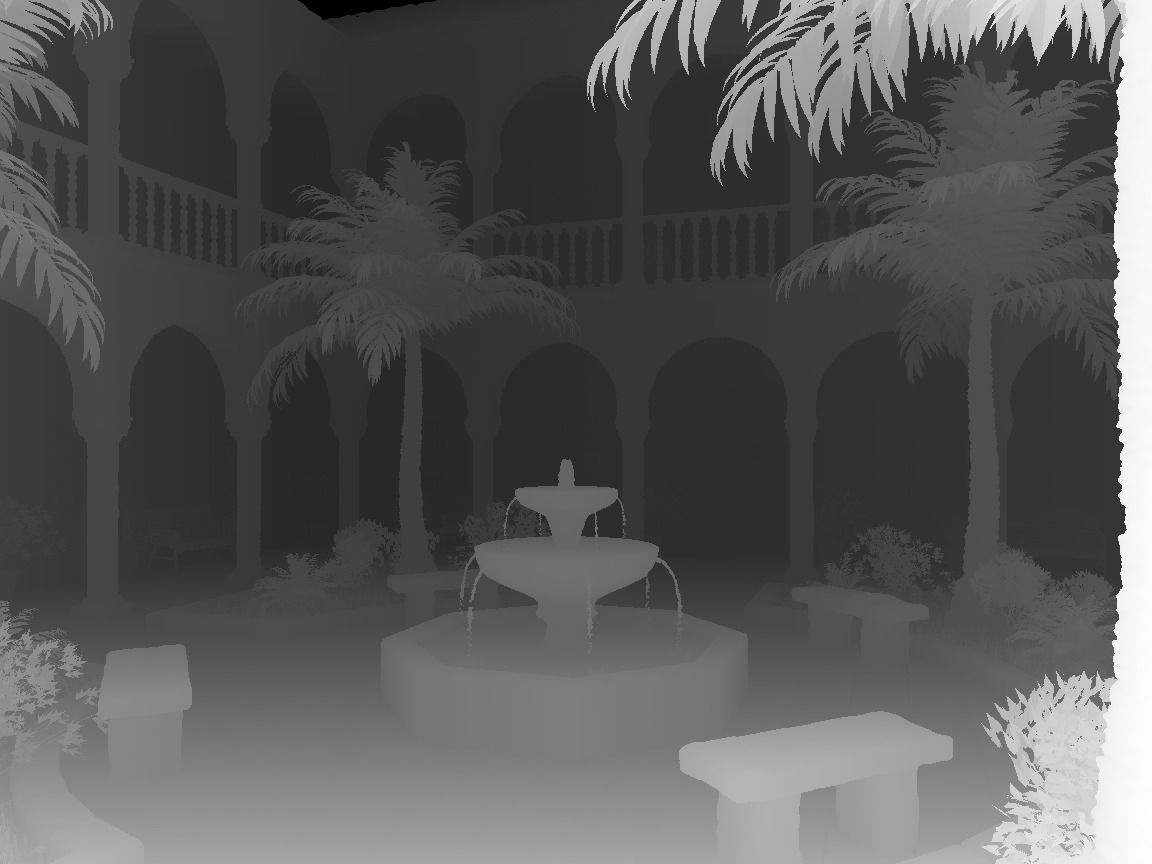
\includegraphics[width=0.7\textwidth]{depth_map_example} }
	\end{minipage}
    \caption{Пример карты глубины.}
	\label{fig:depth_map_example}
\end{figure}


\textit{Карта глубины} $D$ --- матрица размера $h \times w$, состоящая из чисел от 0 до 255,
определяющая расстояние от позиции смотрящего до всех объектов в сцене, 
где значение 255 соответствует положению смотрящего, 128 плоскости экрана, 
а 0 --- <<бесконечности>>. Пример Рис.~\ref{fig:depth_map_example}.

\textit{Последовательность карт глубины} $\{D_t\}_{t=0}^N$ --- конечный упорядоченный 
набор карт глубины одинаковых размеров, которые используются алгоритмом конвертации 
для извлечения информации о расположении объектов в сцене.

\textit{Конвертированное стереовидео} $𝑆$ --- упорядоченная пара видеопоследовательностей 
($\{L_t\}_{t=0}^N$,$\{R_t\}_{t=0}^N$), совпадающих по количеству кадров и размеру кадров, 
где $\{L_t\}_{t=0}^N$ --- это снятая видеопоследовательность, а $\{R_t\}_{t=0}^N$ --- 
полученная на основании $\{L_t\}_{t=0}^N$ и $\{D_t\}_{t=0}^N$, сконвертированная последовательность. 
Видеопоследовательности называются левым и правым ракурсом соответственно.

\textit{Оценка} $q$ --- действительное неотрицательное число $q \in \mathbb{R}^{+} \cup \{0\}$, 
пропорциональное величине заметности артифакта в стереопаре.

Постановка задачи:

\begin{enumerate}
	\item На вход алгоритму, реализующему разрабатываемый метод, подаётся конвертированное стереовидео $𝑆$, а также дополнительно может быть передана последовательность карт глубины $\{D_t\}_{t=0}^N$.
	\item Выходом алгоритма является набор оценок $\{q_t\}_{t=0}^N$, соответствующих кадрам входящей стерео видеопоследовательности.
\end{enumerate}

\subsection{Требования к методу}

Разрабатываемый метод должен быть применим для анализа полнометражных стереоскопических фильмов. Соответственно, он должен удовлетворять следующим требованиям:

\begin{itemize}
	\item Способность находить сцены с заметными артифактами, 
	находящимися в областях салиентного движения.
	\item Низкая доля ошибок первого рода (пропуск сцены) при приемлемой доле 
	ошибок второго рода (ложное срабатывание). Ошибки второго рода менее существенны, 
	так как, если ложных срабатываний не очень много, их можно исключить 
	при ручном просмотре обнаруженных сцен.
	\item Высокая скорость работы на видеопоследовательностях высокого разрешения 
	вплоть до $1920 \times 1080$. Требуется для того, чтобы анализ 
	полнометражного стереоскопического фильма занимал приемлемое время.
	\item Устойчивость к другим типам артифактов, главным из которых является отсутствие глубины в сцене (сцена выглядит плоской, либо присутствует только некоторый градиент по глубине).
\end{itemize}

\subsection{Цели дипломной работы}

Целью дипломной работы является разработка метода, решающего поставленную задачу 
с минимальной долей ошибок первого рода (артифакт не обнаружен) и 
с приемлемой долей ошибок второго рода (ложное срабатывание).

В рамках дипломной работы предполагается решить следующие задачи:

\begin{enumerate}
	\item Провести обзор предметной области алгоритмов оценки качества конвертированного стереовидео.
	\item Разработать метод поиска несоответствий границ объектов между результатом 2D-3D конвертации 
	и используемыми картами глубины, учитывая требования данной задачи.
	\item Разработать алгоритм, реализующий метод, и провести его экспериментальную оценку на соответствие требованиям решаемой задачи.
	\item Произвести массовый анализ реальных стереоскопических фильмов на предмет наличия движущихся объектов, слитых с фоном.
\end{enumerate}


\newpage
\section{Обзор предметной области}
% Обзор должен содержать явно сформулированные цели и критерии сравнения, которые 
% должны коррелировать с требованиями к искомому решению исходной задачи. 
% В конце обзора должны быть сформулированы выводы.

\subsection{Методы оценки качества 2D видеопоследовательностей}

Многие годы ислледователи изучали качество 2D видеопоследовательностей. 
Wang~\cite{wang2006survey} предложил исчерпывающий обзор основных подходов в данной области.
Самым популярным методом является \textbf{Peak-Signal-to-Noise-Ratio (PSNR)}:
\begin{equation*}
	MSE = \frac{\sum_{i=0}^{h}\sum_{j=0}^{w}[I(i, j) - I'(i, j)]^2}{h \cdot w},
\end{equation*}
\begin{equation}
	PSNR = 20 \cdot \log_{10}(\frac{255}{MSE}),
\end{equation}
где $I$, $I'$ два изображения, которые сравниваются. Чем выше значение $PSNR$, 
тем больше похожи изображения, $PSNR \equiv +\infty$ соответствует одинаковым изображениям. 
Метод \textbf{Structural Similarity Index (SSIM)} многими ислледователями был принят, 
как основной метод оценки качества приближающий субъективную оценку. Данный метод встречается
практически в каждой статье и описывается следующим уравнением:
\begin{equation}
	SSIM = \frac{(2\bar{x}\bar{y} + C_1)(2\sigma_{xy} + C_	2)}{[\bar{x}^2 + \bar{y}^2 + C_1](\sigma_x^2 + \sigma_y^2 + C_2)},
\end{equation} 
где $\bar{x}$, $\bar{y}$, $\sigma_x$, $\sigma_y$, $\sigma_{xy}$ --- средние значение 
для первого изображения, средние значение для второго изображения, дисперсия для $x$, 
дисперсия для $y$, ковариация $x$ и $y$; $C_1$, $C_2$ --- константы. Значение $SSIM$ 
высчитывается с помощью скользящего окна размером $11 \times 11$ с весами Гауссового ядра, 
а итоговое значение для двух изображений --- это среднее по всем высчитанным окнам.

\subsection{Методы оценки качества стереоскопического видео}

Основными направлениями исследований в области оценки качества стереоскопического видео 
являются множественные несоответствия между ракурсами и временная стабильность 
динамического диапазона глубины. Voronov в соавторстве~\cite{voronov2012towards} предложил
способ нахождения разницы между ракурсами по цвету, резкости, 
а также различных геометрических искажений. В статье~\cite{akimov2012automatic} авторами 
был предложен метод нахождения перепутанных ракурсов в стереовидео. 

Артифакты, влияющие на качество конвертированного стереоскопического видео, более 
разнообразны и менее изучены в научных кругах. Bokov в соавторстве~\cite{bokov2014automatic} 
предложил алгоритм поиска трех основных проблем, возникающих при конвертации:
\begin{itemize}
	\item Резкость границ объектов,
	\item Эффект кулисности,
	\item Плоские сцены.
\end{itemize}
Ожидаемо, данный алгоритм подходит для обнаружения проблем только для тех объектов, 
которые присутствуют на карте глубины. В данной дипломной работе предлагается 
дополнительный метод, расширяющий возможности оценки качество конвертированного стереовидео,
позволяющий находить объекты переднего планы частично или полностью отсутствующие
на используемых картах глубины.

\subsection{Обзор базовых алгоритмов}

Предлагаемый метод является композицией двух крупных областей исследований: извлечение структуры 
сцены на основании информации о движении, а также алгоритмов сопоставления краев и контуров 
между двумя картами границ. Обе области достаточно хорошо изучены.

Многие методы извлечения структуры сцены из движения предполагают минимизацию функции энергии
с членом, отвечающим амплитуде движения, извлеченной из сцены. Яркий 
представитель~\cite{zhang2009consistent} дополнительно учитывает ограничение, 
обеспечивающее временную стабильность, а также уточняют положение объектов с помощью ротации 
в пространстве плоскостей, соответствующих цветовым сегментам кадра, в сторону уменьшения энергии.
Такой подход позволяет извлекать карты глубины высокого качества, обладающих временной стабильностью.
Однако временная сложность алгоритма не подходит для решения прикладных задач, в частности 
для анализа полнометражного стереоскопического фильма. Недавно предложенный метод
фильтрации~\cite{he2013guided}, сохраняющий края объектов, позволил положить в основу разрабатываемого
метода менее вычислительно сложный подход: изначально извлекается сырая карта амплитуды движения 
с помощью блочного алгоритма оценки векторов движения~\cite{simonyan2008fast}, а затем улучшается
путем свертки фильтром, сохраняющим границы объектов.

Для решения задачи сопоставления контуров, было рассмотрено несколько современных точных алгоритмов
сопоставления замкнутых контуров. Например, Xu в соавторстве~\cite{xu20092d} предложил метод,
основанный на дексрипторе гибкости контуров. Расширение на случай не замкнутых контуров возможно, 
однако потребует использования не самого точного алгоритма водоразделов~\cite{roerdink2000watershed}, что повлечет значительное увеличение ошибок второго рода. Другой 
подход~\cite{felzenszwalb2007hierarchical} заключается в использовании особой структуры ---
иерархического дерево форм. К сожалению, данный метод не расширяется на разрывные контура, 
что критично в нашем случае, так как оценка карт амплитуды движения не является идеальной и содержит
в том числе большое количество контуров не являющихся непрерывными и замкнутыми. Таким образом, 
в ходе анализа предметной области было решено использовать менее точный, но более устойчивый
к качеству анализируемых контуров, метод схожий к distance transform~\cite{borgefors1986distance}.

\subsection{Выводы}

В ходе обзора предметной области были сделаны следующие выводы о структуре проектируемого метода:

\begin{itemize}
	\item Использовать блочный алгоритм оценки векторов движения с последующим улучшением
	путем свертки фильтром, сохраняющим границы объектов. Такой подход не даст самой высокой 
	точности, однако позволит провести анализ за разумное время.
	\item Использовать похожий на distance transform алгоритм сопоставления контуров, устойчивый
	к входным данным, потенциально поврежденным, как следствие неидельности используемых методов.
\end{itemize}

\newpage
\section{Предложенный метод}

\begin{figure}[!h]
	\begin{minipage}[b]{1.0\linewidth}
		\centering
		\centerline{ 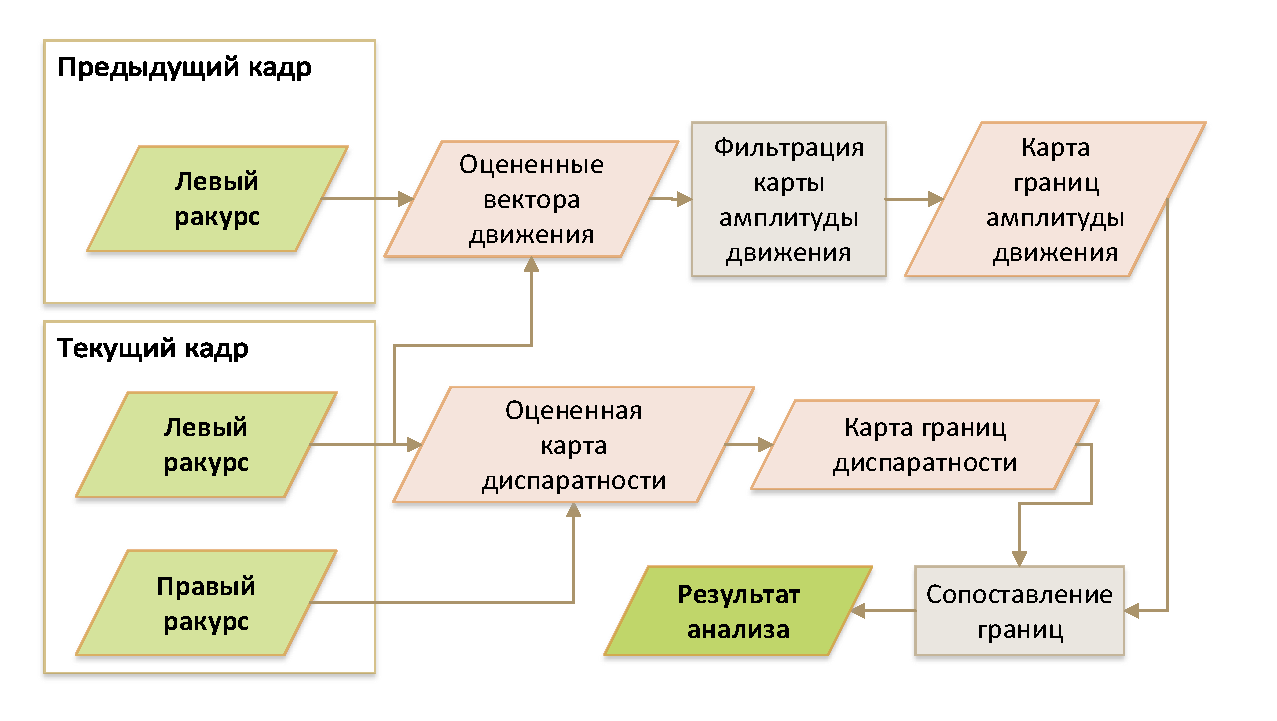
\includegraphics[width=\textwidth]{full_pipeline_rus.pdf} }
	\end{minipage}
    \caption{ Схема предлагаемого метода. Шаг оценки карты диспаратности 
    	может быть опущен в случае, когда доступна оригинальная карта глубины. }
	\label{fig:full}
\end{figure}

\begin{figure}[!h]
	\begin{minipage}[b]{0.49\linewidth}
		\centering
		\centerline{ 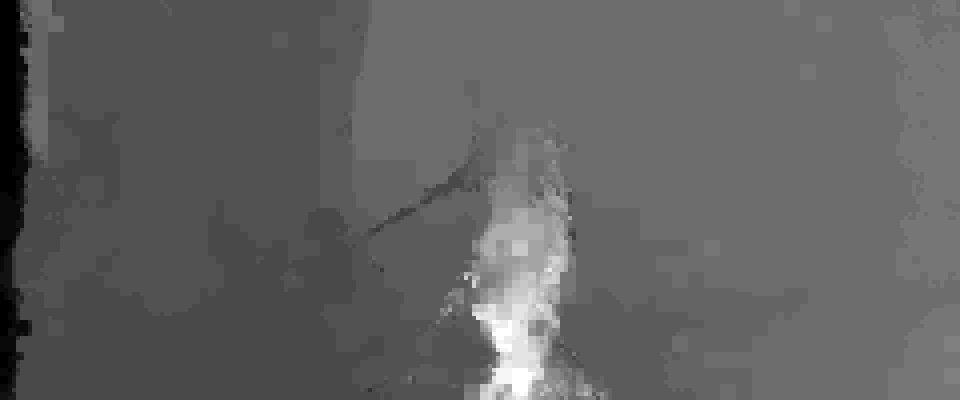
\includegraphics[width=\linewidth]{motionx} }
		\centerline{\scriptsize{(a) Horizontal-motion strength map}}\medskip
	\end{minipage}%
	\hfill
	\begin{minipage}[b]{0.49\linewidth}
		\centering
		\centerline{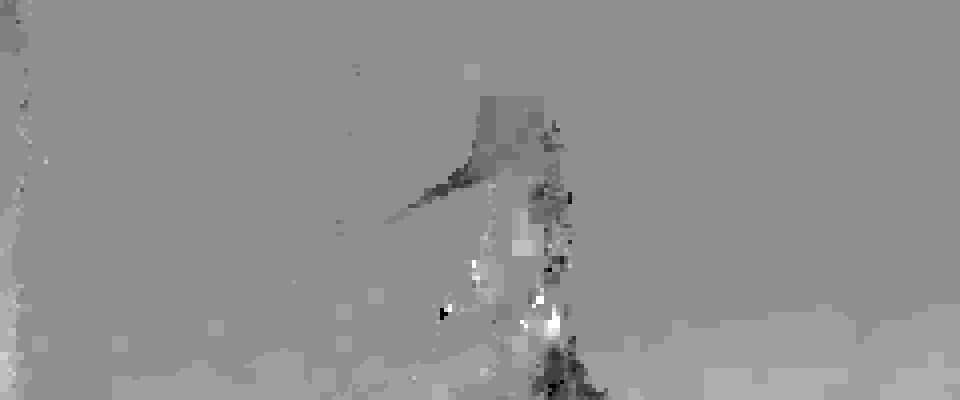
\includegraphics[width=\linewidth]{motiony} }
		\centerline{\scriptsize{(b) Vertical-motion strength map}}\medskip
	\end{minipage}
	\begin{minipage}[b]{0.49\linewidth}
		\centering
		\centerline{ 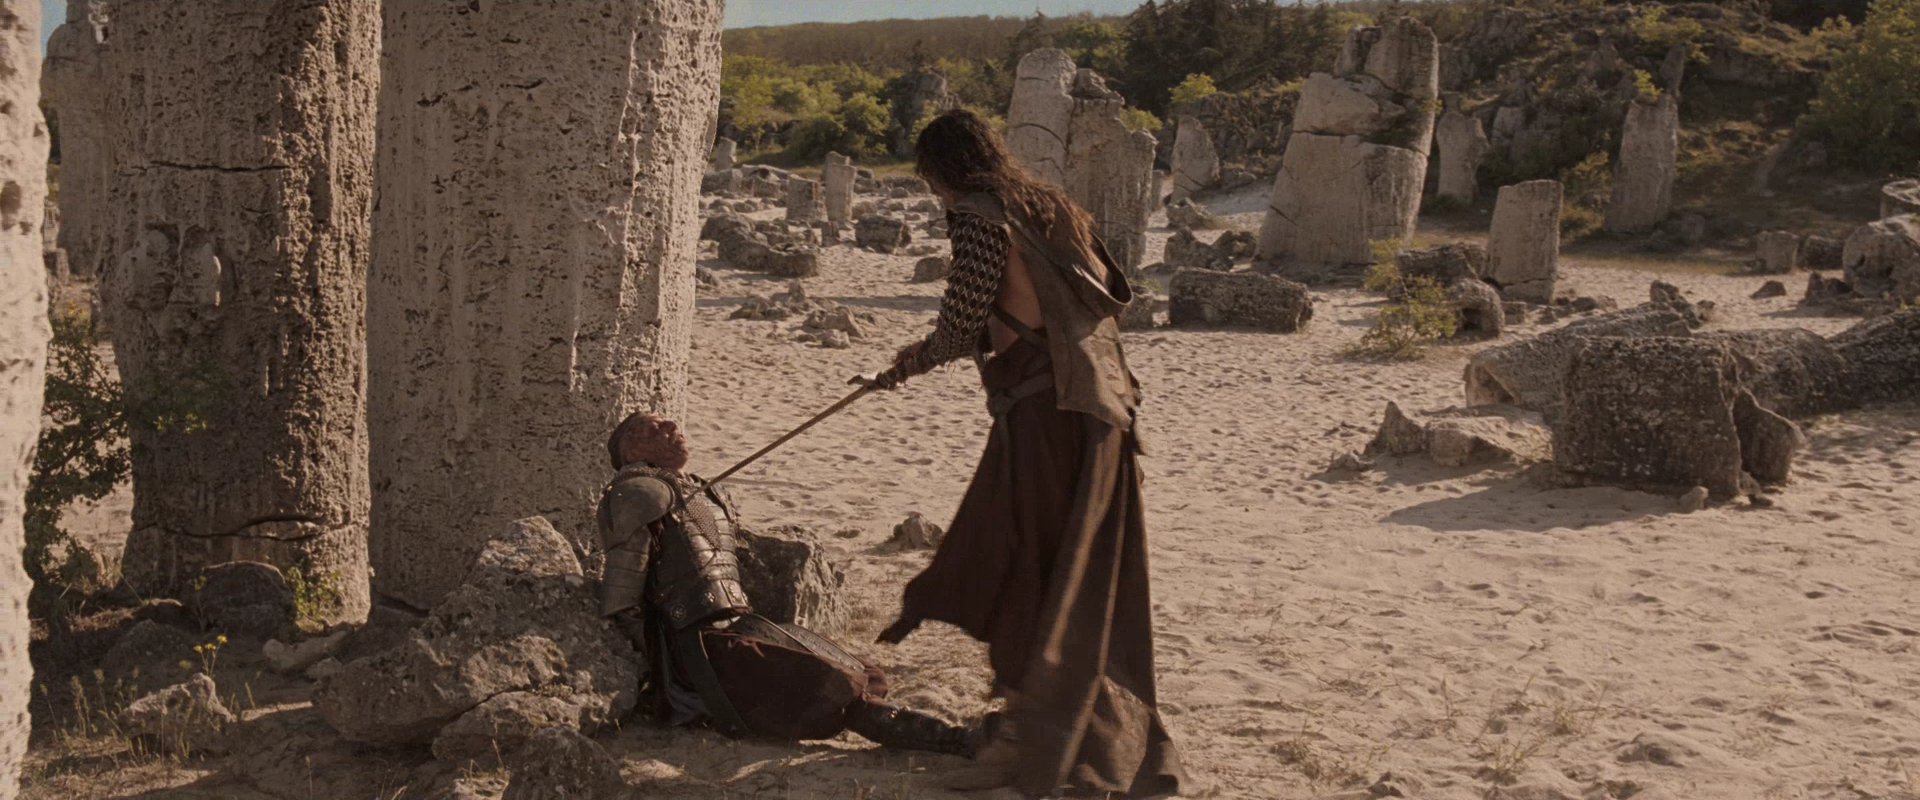
\includegraphics[width=\linewidth]{src} }
		\centerline{\scriptsize{(c) Source left view}}\medskip
	\end{minipage}%
	\hfill
	\begin{minipage}[b]{0.49\linewidth}
		\centering
		\centerline{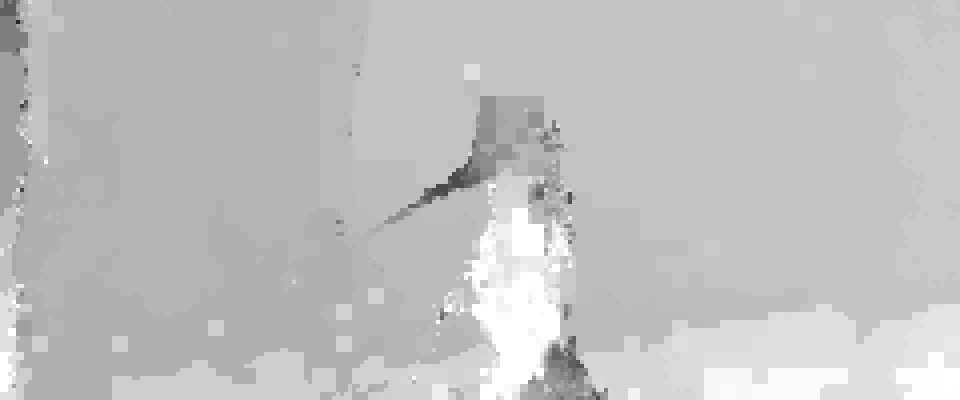
\includegraphics[width=\linewidth]{merged} }
		\centerline{\scriptsize{(d) Overall motion-strength map}}\medskip
	\end{minipage}
	\begin{minipage}[b]{\linewidth}
	\caption{Example maps of horizontal~(a) and vertical~(b) motion extracted
        using a block-based motion-estimation algorithm~\cite{simonyan2008fast} for the source frame~(c).
        The results  are combined into an overall motion-strength map~(d).}
    \label{fig:merged}
    \end{minipage}
\end{figure}

\begin{figure}[!h]
	\begin{minipage}[b]{1.0\linewidth}
		\centering
		\centerline{ 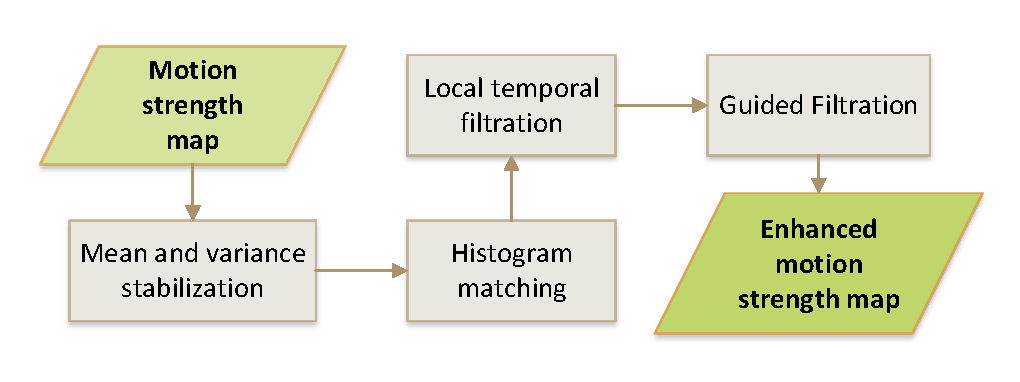
\includegraphics[width=\textwidth]{dfm_pipeline.pdf} }
	\end{minipage}
    \caption{Pipeline of spatio-temporal filtering. This approach enables us to enhance the rough
        motion-intensity map that we obtain from the motion-estimation algorithm.}
	\label{fig:dfm}
\end{figure}

\begin{figure}[!h]
	\begin{minipage}[b]{0.49\linewidth}
		\centering
		\centerline{ 
\includegraphics[width=\linewidth]{mean_and_variance} }
		\centerline{(а) Результат стабилизации}
		\centerline{среднего и дисперсии}\medskip
	\end{minipage}%
	\hfill
	\begin{minipage}[b]{0.49\linewidth}
		\centering
		\centerline{
\includegraphics[width=\linewidth]{histogram_matching} }
		\centerline{(б) Результат сопоставления}
		\centerline{гистограмм}\medskip
	\end{minipage}
	\hfill
	\begin{minipage}[b]{0.49\linewidth}
		\centering
		\centerline{ 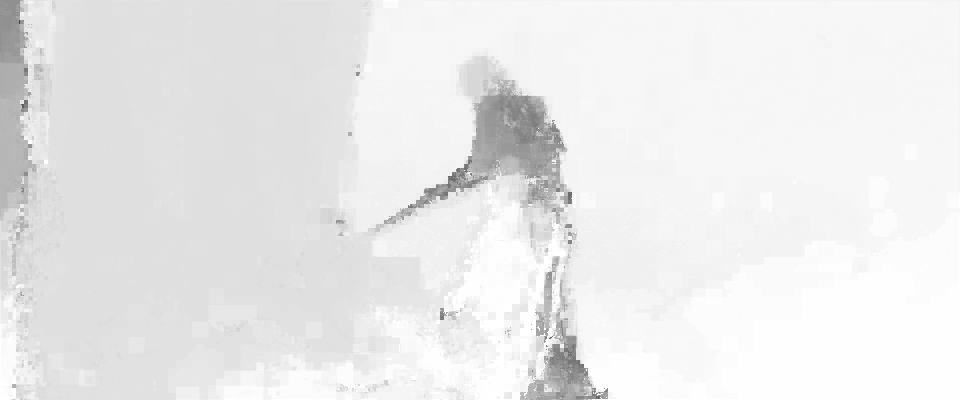
\includegraphics[width=\linewidth]{stabilization} }
		\centerline{(в) Результат временной}
		\centerline{фильтрации}\medskip
	\end{minipage}%
	\hfill
	\begin{minipage}[b]{0.49\linewidth}
		\centering
		\centerline{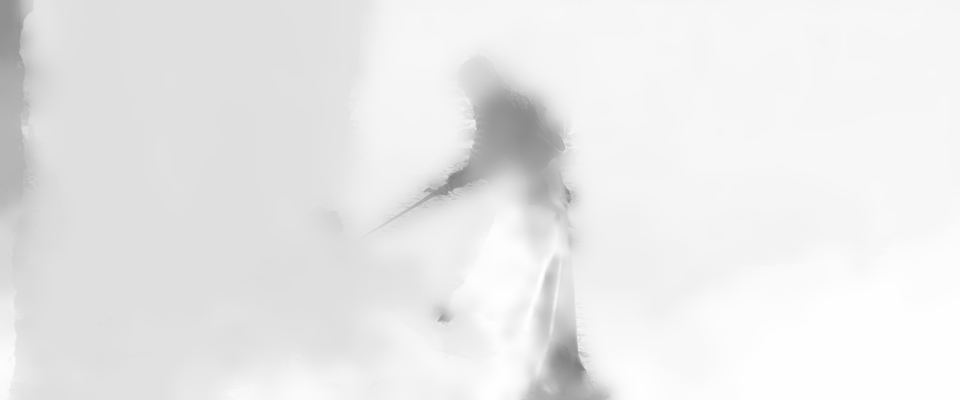
\includegraphics[width=\linewidth]{guided_filtration} }
		\centerline{(г) Результат применения}
		\centerline{Guided filter}\medskip
	\end{minipage}
	\begin{minipage}[b]{\linewidth}
    \caption{ Примеры, иллюстрирующие каждый промежуточный этап конвейера
    	просранственно-временных фильтраций из Рис.~\ref{fig:dfm}.}
    \label{fig:filtered}
    \end{minipage}
\end{figure}


Fig.~\ref{fig:full} shows the scheme of the proposed method for detecting inconsistencies 
between object motion and the depth map used in converting 2D to 3D video. The method input is S3D 
video converted from 2D and, optionally, the depth map used during conversion. The method outputs 
a per-frame score that can be interpreted as a perimeter of objects that were absent from the depth map. 
It comprises the following steps:
\begin{enumerate}
	\item Estimate left-view motion vectors between previous and current frames.
	\item Estimate disparity map between left and right view (if no depth map is available). 
	We can use a disparity map instead of a depth map because our method requires only 
	information about depth-map edges, which match the disparity-map edges.
	\item Compute motion-strength maps using a motion-vector field refined by temporal 
	and spatial processing to improve its temporal coherence.
	\item Perform edge matching between motion-strength and depth maps.
	\item Compute area of motion-strength-map edges that are absent from the depth map. 
	This area is the final frame score.
\end{enumerate}

\begin{figure}[t]
	\begin{minipage}[b]{0.49\linewidth}
		\centering
		\centerline{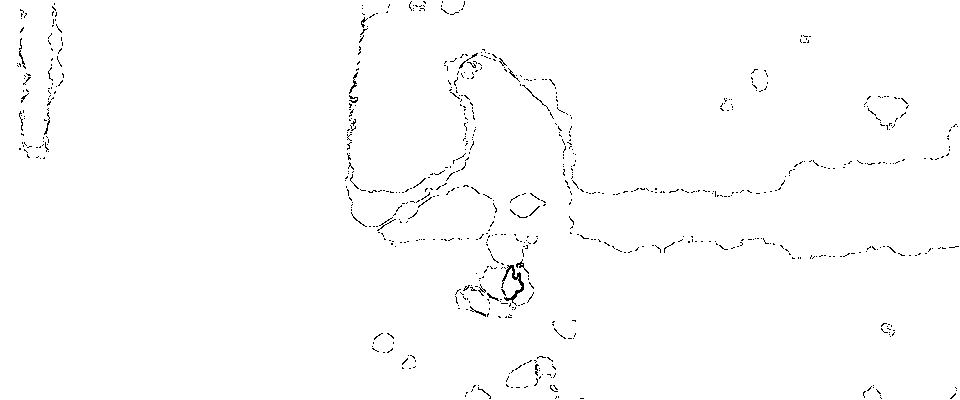
\includegraphics[width=\textwidth]{disparity_contours} }
		\centerline{(а) Границы, извлеченные}
		\centerline{из карты диспаратности}\medskip
	\end{minipage}
	\begin{minipage}[b]{0.49\linewidth}
		\centering
		\centerline{ 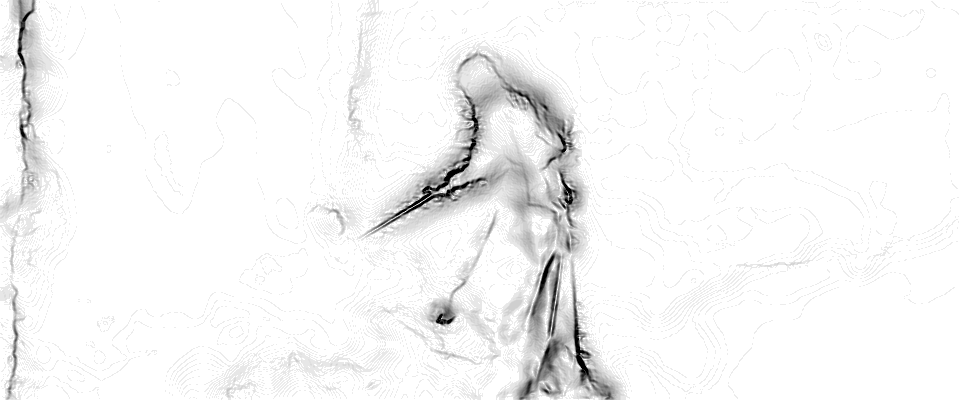
\includegraphics[width=\textwidth]{drop_contours} }
		\centerline{(б) Границы, извлеченные}
		\centerline{из карты амплитуды движения}\medskip
	\end{minipage}
	\hfill
	\begin{minipage}[b]{0.49\linewidth}
		\centering
		\centerline{ 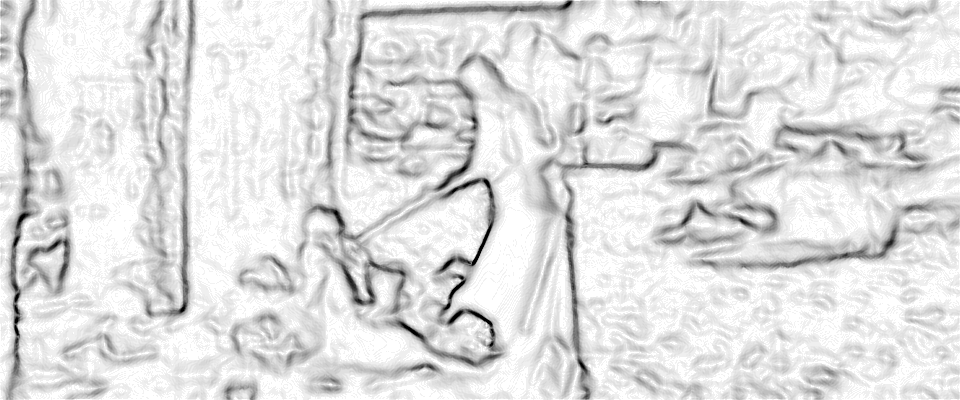
\includegraphics[width=\textwidth]{src_contours} }
		\centerline{(в) Границы, извлеченные}
		\centerline{из исходного кадра}\medskip
	\end{minipage}
	\hfill
	\begin{minipage}[b]{0.49\linewidth}
		\centering
		\centerline{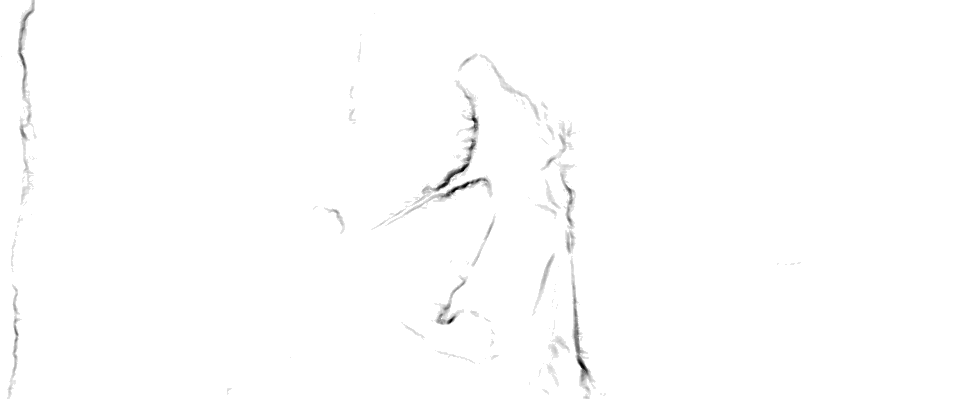
\includegraphics[width=\textwidth]{dfm_contours} }
		\centerline{(г) Пересечение границ}\medskip
		\centerline{движения~(б) и исходных~(в)}\medskip
	\end{minipage}
	\begin{minipage}[b]{\linewidth}
    \caption{Границы, извлеченные из карты диспаратности~(а), улучшенной карты
    	амплитуды движения~(б), и исходного кадра после применения фильтрации,
    	сохраняющей контуры объектов~(в). Пересечение границ карты интенсивности
    	движения и исходного кадра изображено на~(г).}
    \label{fig:edges}
    \end{minipage}
\end{figure}


To extract both the motion and disparity maps, we employ the block-based matching approach 
described in~\cite{simonyan2008fast}. To estimate a confidence value for the resulting maps, 
we use a left\slash right-consistency constraint (LRC)~\cite{egnal2004stereo} 
(which takes the form of a previous\slash current-consistency constraint in the case of motion estimation).

We compute motion-strength map $M$ as the magnitude of a motion-vector field (see Fig.~\ref{fig:merged}~(a) and (b)).
Then, to improve the temporal coherence of the motion-strength map, we apply the pipeline
of temporal and spatial filters shown in Fig.~\ref{fig:dfm}.

We begin by applying a linear transform to the motion-strength map; this transform sets the minimum value 
in the map equal to 0 and the maximum value equal to 1 (i.e., auto levels). Fig.~\ref{fig:merged}~(d) shows 
an example intermediate result for this step. Owing to changes in camera and object velocity as well as 
errors in the motion-vector field, the resulting motion-strength map contains a good deal of flickering. 
To reduce this effect, we set the mean and standard deviation of each frame equal to the means 
of these values computed over the previous $n$ frames (our experiments used $n = 10$):
\begin{equation}
M_{i}^{'k} = \frac{\mathsf{Std}_{k-n}^{k-1}}{\mathsf{Std}\left[M^k\right]} \left( M_i^k - \mathsf{E}\left[M^k\right]\right) + \mathsf{E}_{k-n}^{k-1}
\end{equation}
Here, $\mathsf{E}$ and $\mathsf{Std}$ are the mean and standard deviation, respectively; 
$M^k_i$ is pixel $i$ of the motion-strength map for frame $k$; and $\mathsf{E}_{k-n}^{k-1}$ and 
$\mathsf{Std}_{k-n}^{k-1}$ are the temporal mean and standard deviation, respectively. 
We calculate these last two values as follows:
\begin{equation}
\mathsf{E}_{k-n}^{k-1} =  \frac{1}{\#} \sum_{i}\left(\frac{1}{n}\sum_{p=k-n}^{k-1}M_i^p\right)
\label{fm:temp_mean}
\end{equation}
\begin{equation}
\mathsf{Std}_{k-n}^{k-1} = \sqrt{\frac{1}{\# - 1} \sum_{i}\left(\frac{1}{n}\sum_{p=k-n}^{k-1}M_i^p - \mathsf{E}_{k-n}^{k-1}\right)^2}
\label{fm:temp_std}
\end{equation}

In (\ref{fm:temp_mean}) and (\ref{fm:temp_std}) $\#$ denotes the number of pixels in the frame.
Fig.~\ref{fig:filtered}~(a) shows an intermediate result from this step. As a final global transform 
we apply histogram matching~\cite{fecker2007time} to the sequence of motion-strength maps. 
This transform makes the histogram of each these maps match the mean 
histogram of the previous $n$ frames. An example result appears in Fig.~\ref{fig:filtered}~(b).

To remove any local flickering that persists after the global transforms, we use  the
temporal-stabilization method proposed in~\cite{matyunin2011temporal} 
(see the example result in Fig.~\ref{fig:filtered}~(c)).

\begin{figure}[t]
	\begin{minipage}[b]{0.49\linewidth}
		\centering
		\centerline{ 
\includegraphics[width=\textwidth]{disp} }
		\centerline{\scriptsize{(a) Estimated disparity map }}\medskip
	\end{minipage}
	\hfill
	\begin{minipage}[b]{0.49\linewidth}
		\centering
		\centerline{
\includegraphics[width=\textwidth]{wmf} }
		\centerline{\scriptsize{(b) Enhanced disparity map}}\medskip
	\end{minipage}
	\begin{minipage}[b]{1\linewidth}
		\centering
		\centerline{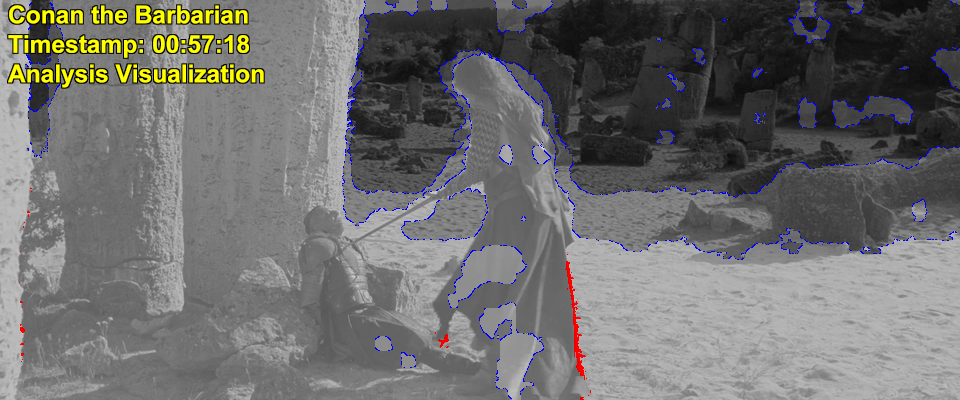
\includegraphics[width=\textwidth]{visualization} }
		\centerline{\scriptsize{(c) Visualization of final result }}
	\end{minipage}
    \caption{Examples of a disparity map before~(a) and after~(b) weighted-median
        filtering. The resulting visualization~(c) that we offer to content
        creators is a disparity map overlaid on the source frame. We use blue to mark
        the disparity edges and red to mark any inconsistencies
        between motion- and disparity-map edges.}
	\label{fig:disp}
\end{figure}


Finally, to improve the consistency of the motion-strength-map edges with image edges and 
to fill areas of low confidence, we use a guided filter~\cite{he2013guided} with the input frame 
as the guide. Fig.~\ref{fig:filtered}~(d) shows an example of the final motion-strength map.

Now consider the case where no depth map is available and the disparity map is estimated using 
a block-based matching algorithm.To improve the disparity map we apply a fast version of 
the weighted-median filter described in~\cite{zhang2014100+}. This filter refines the object contours 
and removes extraneous edges from what should be smooth disparity transitions. An example of an estimated 
disparity map before and after filtration appears in Fig.~\ref{fig:disp}~(a) and (b).

We apply a Scharr operator~\cite{jahne1999principles} to both the filtered motion strength-map 
and the depth map to detect their edges. Fig.~\ref{fig:edges}~(a) and (b) shows example edge maps. 
Since the motion-strength edge map contains blurred edges caused by guided filtration, we use 
edge information from the source RGB frame to sharpen them. We cannot, however, use the edge map 
of the source frame as is, since it contains numerous texture edges that are not actual object edges. 
To remove most texture edges we apply scale-aware filtration~\cite{zhang2014rolling} to the source 
frame and extract the edge map from the filtered frame (see Fig.~\ref{fig:edges}~(d)).

Finally, we compute the intersection of the edges we extracted from the motion-strength map ($M$) 
and the filtered source frame ($I$) using the equation below:
\begin{equation}
M_i^{'k} =M_i^k\max_{j  \in B_{r}(i)}(I_j^k)
\end{equation}
Here, $B_{r}(i)$ is the neighborhood of radius $r = 0$ around pixel $i$. We use the same procedure 
with $r = 5$ to refine the disparity map.

To get a final quality score for the current frame, we intersect the edges of the refined motion-strength map 
with the edges of the disparity map using a method inspired by the distance transform. For each pixel 
in the motion-strength edge map we iteratively calculate the distance value:
\begin{equation}
\begin{split}
M_i^{k,0} &= M_i^k, \\
M_i^{k,t} &= M_i^{k,t-1} - \max_{j \in B_t(i)}w(i,j)\frac{\left(\vec{M}_i^{k,t-1}, \vec{D}_j  \right)}{\lVert\vec{D}_j\rVert}
\end{split}
\end{equation}
In this expression, $w(i,j)$ is a distance weight function:
\begin{equation}
w(i,j) = \exp\left(\frac{\lVert i-j \rVert^2}{2\sigma^2}\right)
\end{equation}
Here, $\vec{M}_i^{k,t-1}$ and $\vec{D}_j$ are motion-strength and disparity edge maps extracted using 
a Scharr operator. The resulting map contains only edges that are present in the motion-strength map 
but are missing from the depth map. These edges likely belong to objects that do not appear in the depth map. 
An example of a final result appears with red lines in Fig.~\ref{fig:disp}~(c).

\begin{figure}[!h]
	\begin{minipage}[b]{0.49\linewidth}
		\centering
		\centerline{ 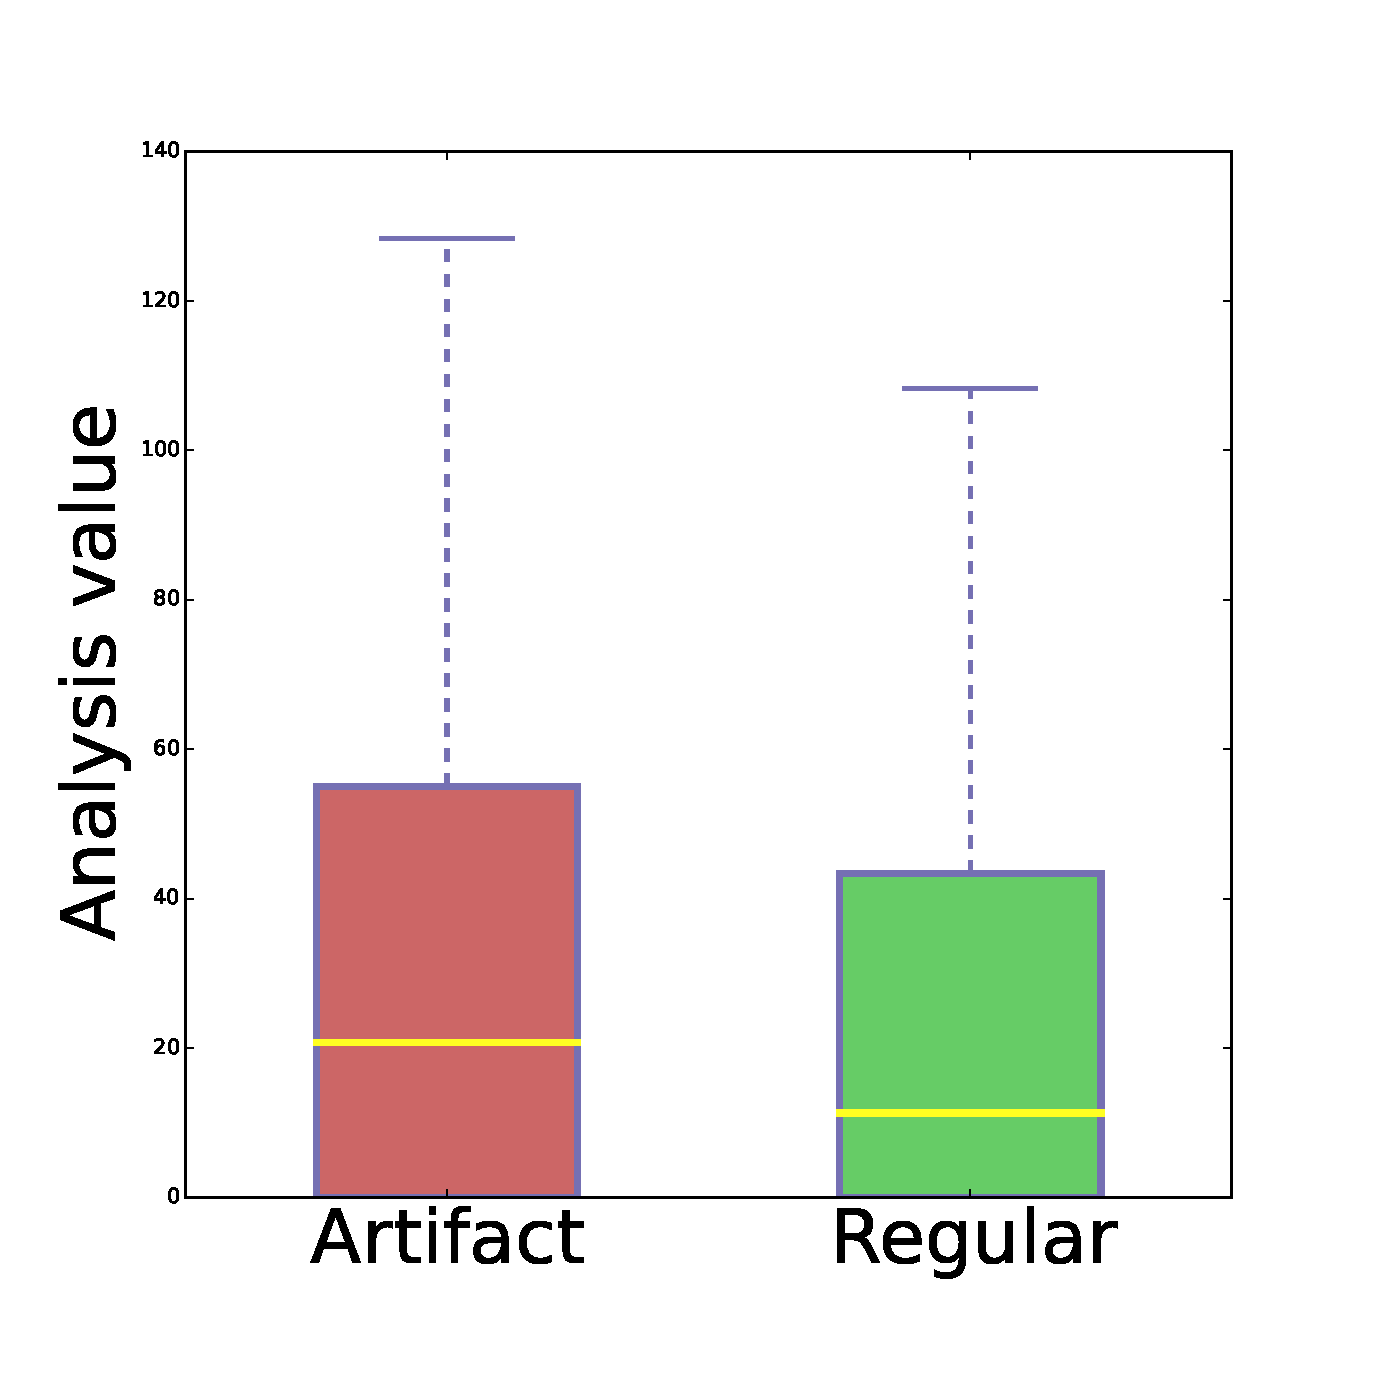
\includegraphics[width=\textwidth]{v1_test} }
		\centerline{\scriptsize{(a) Scores computed using}}
		\centerline{\scriptsize{initial algorithm}}\medskip
	\end{minipage}
	\hfill
	\begin{minipage}[b]{0.49\linewidth}
		\centering
		\centerline{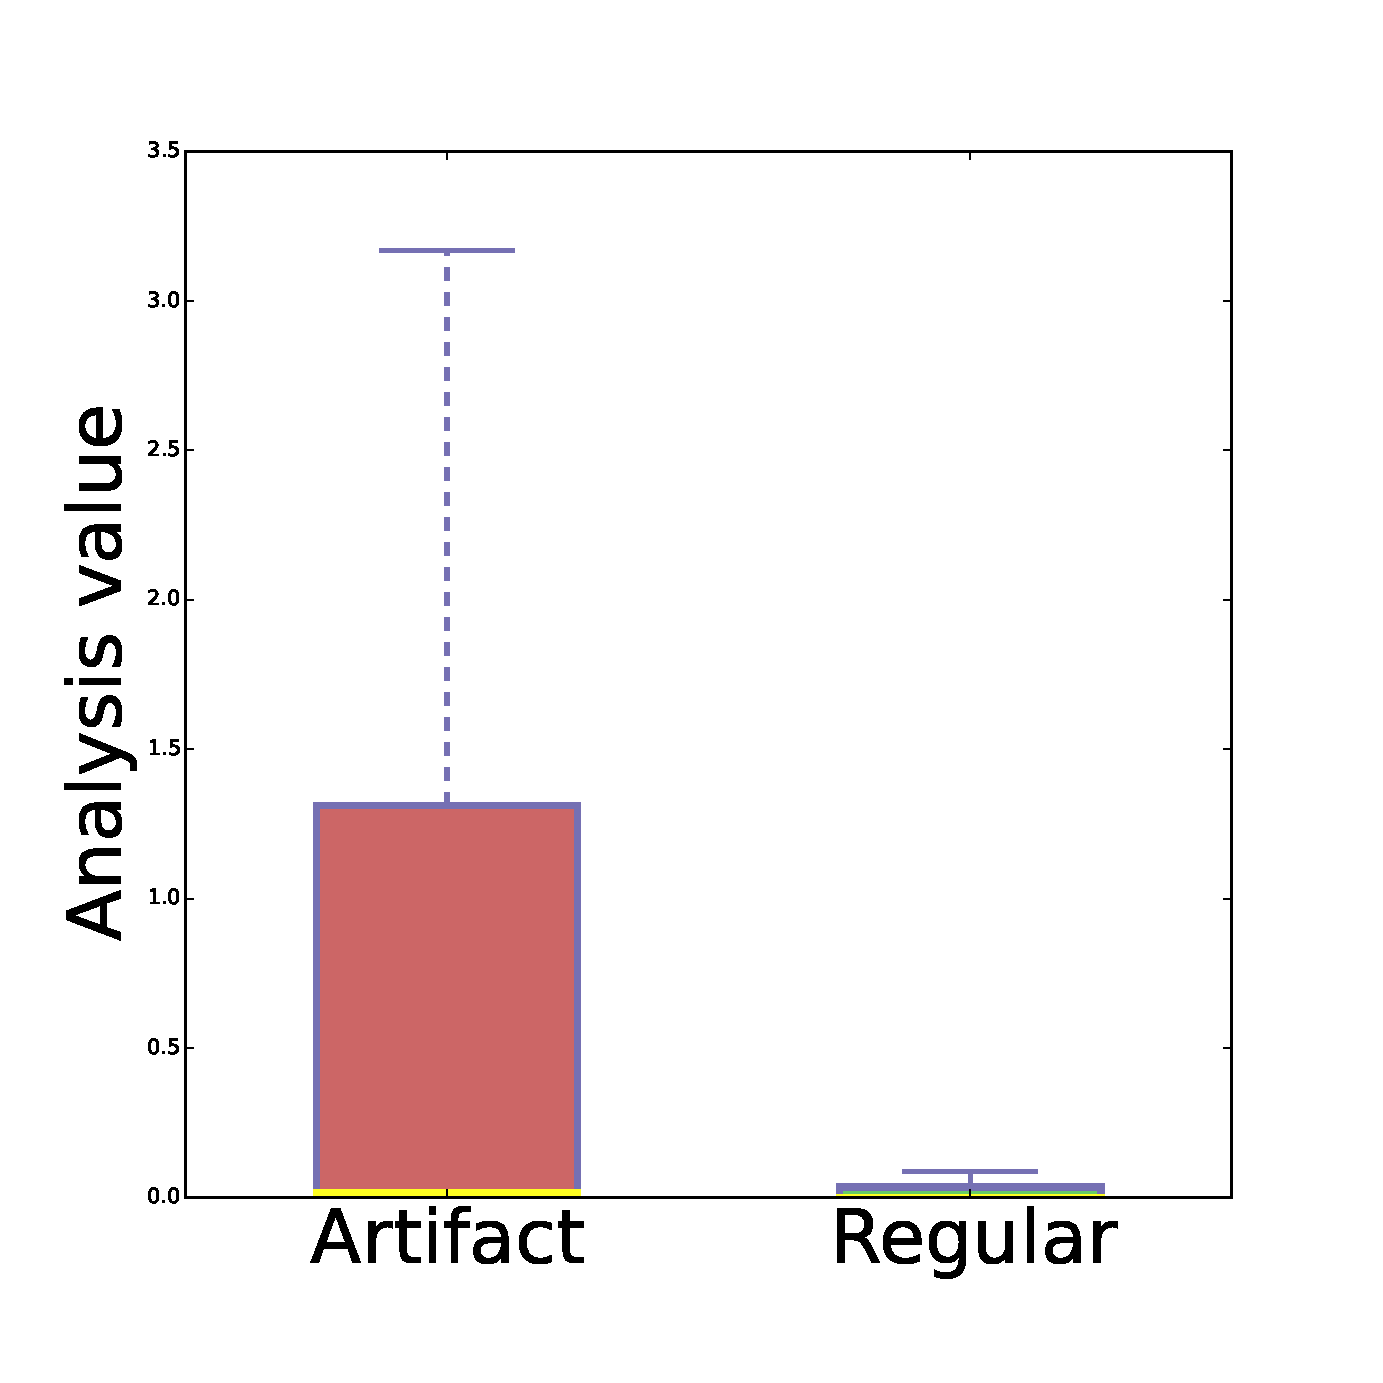
\includegraphics[width=\textwidth]{v2_test} }
		\centerline{\scriptsize{(b) Scores computed using}}
		\centerline{\scriptsize{modified algorithm}}\medskip
	\end{minipage}
    \caption{Mean scores of the initial algorithm~(a) for true- and false-positive
        scenes, as well as mean scores computed for the same scenes using an algorithm modified
        to exclude RGB uniform regions~(b).}
	\label{fig:textureless}
\end{figure}



\newpage
\section{Экспериментальная оценка}

We used the algorithm described in the previous section to evaluate the false-positive ratio for 
a set of five movies. To create a validation data set, we manually classified  the detected frames 
as either true positive or false positive. The data set consisted of 21 true-positive scenes and 
31 false-positive scenes (see Table~\ref{tab:testsample}).

\begin{figure}[!h]
	\begin{minipage}[b]{1.0\linewidth}
		\centering
		\centerline{ 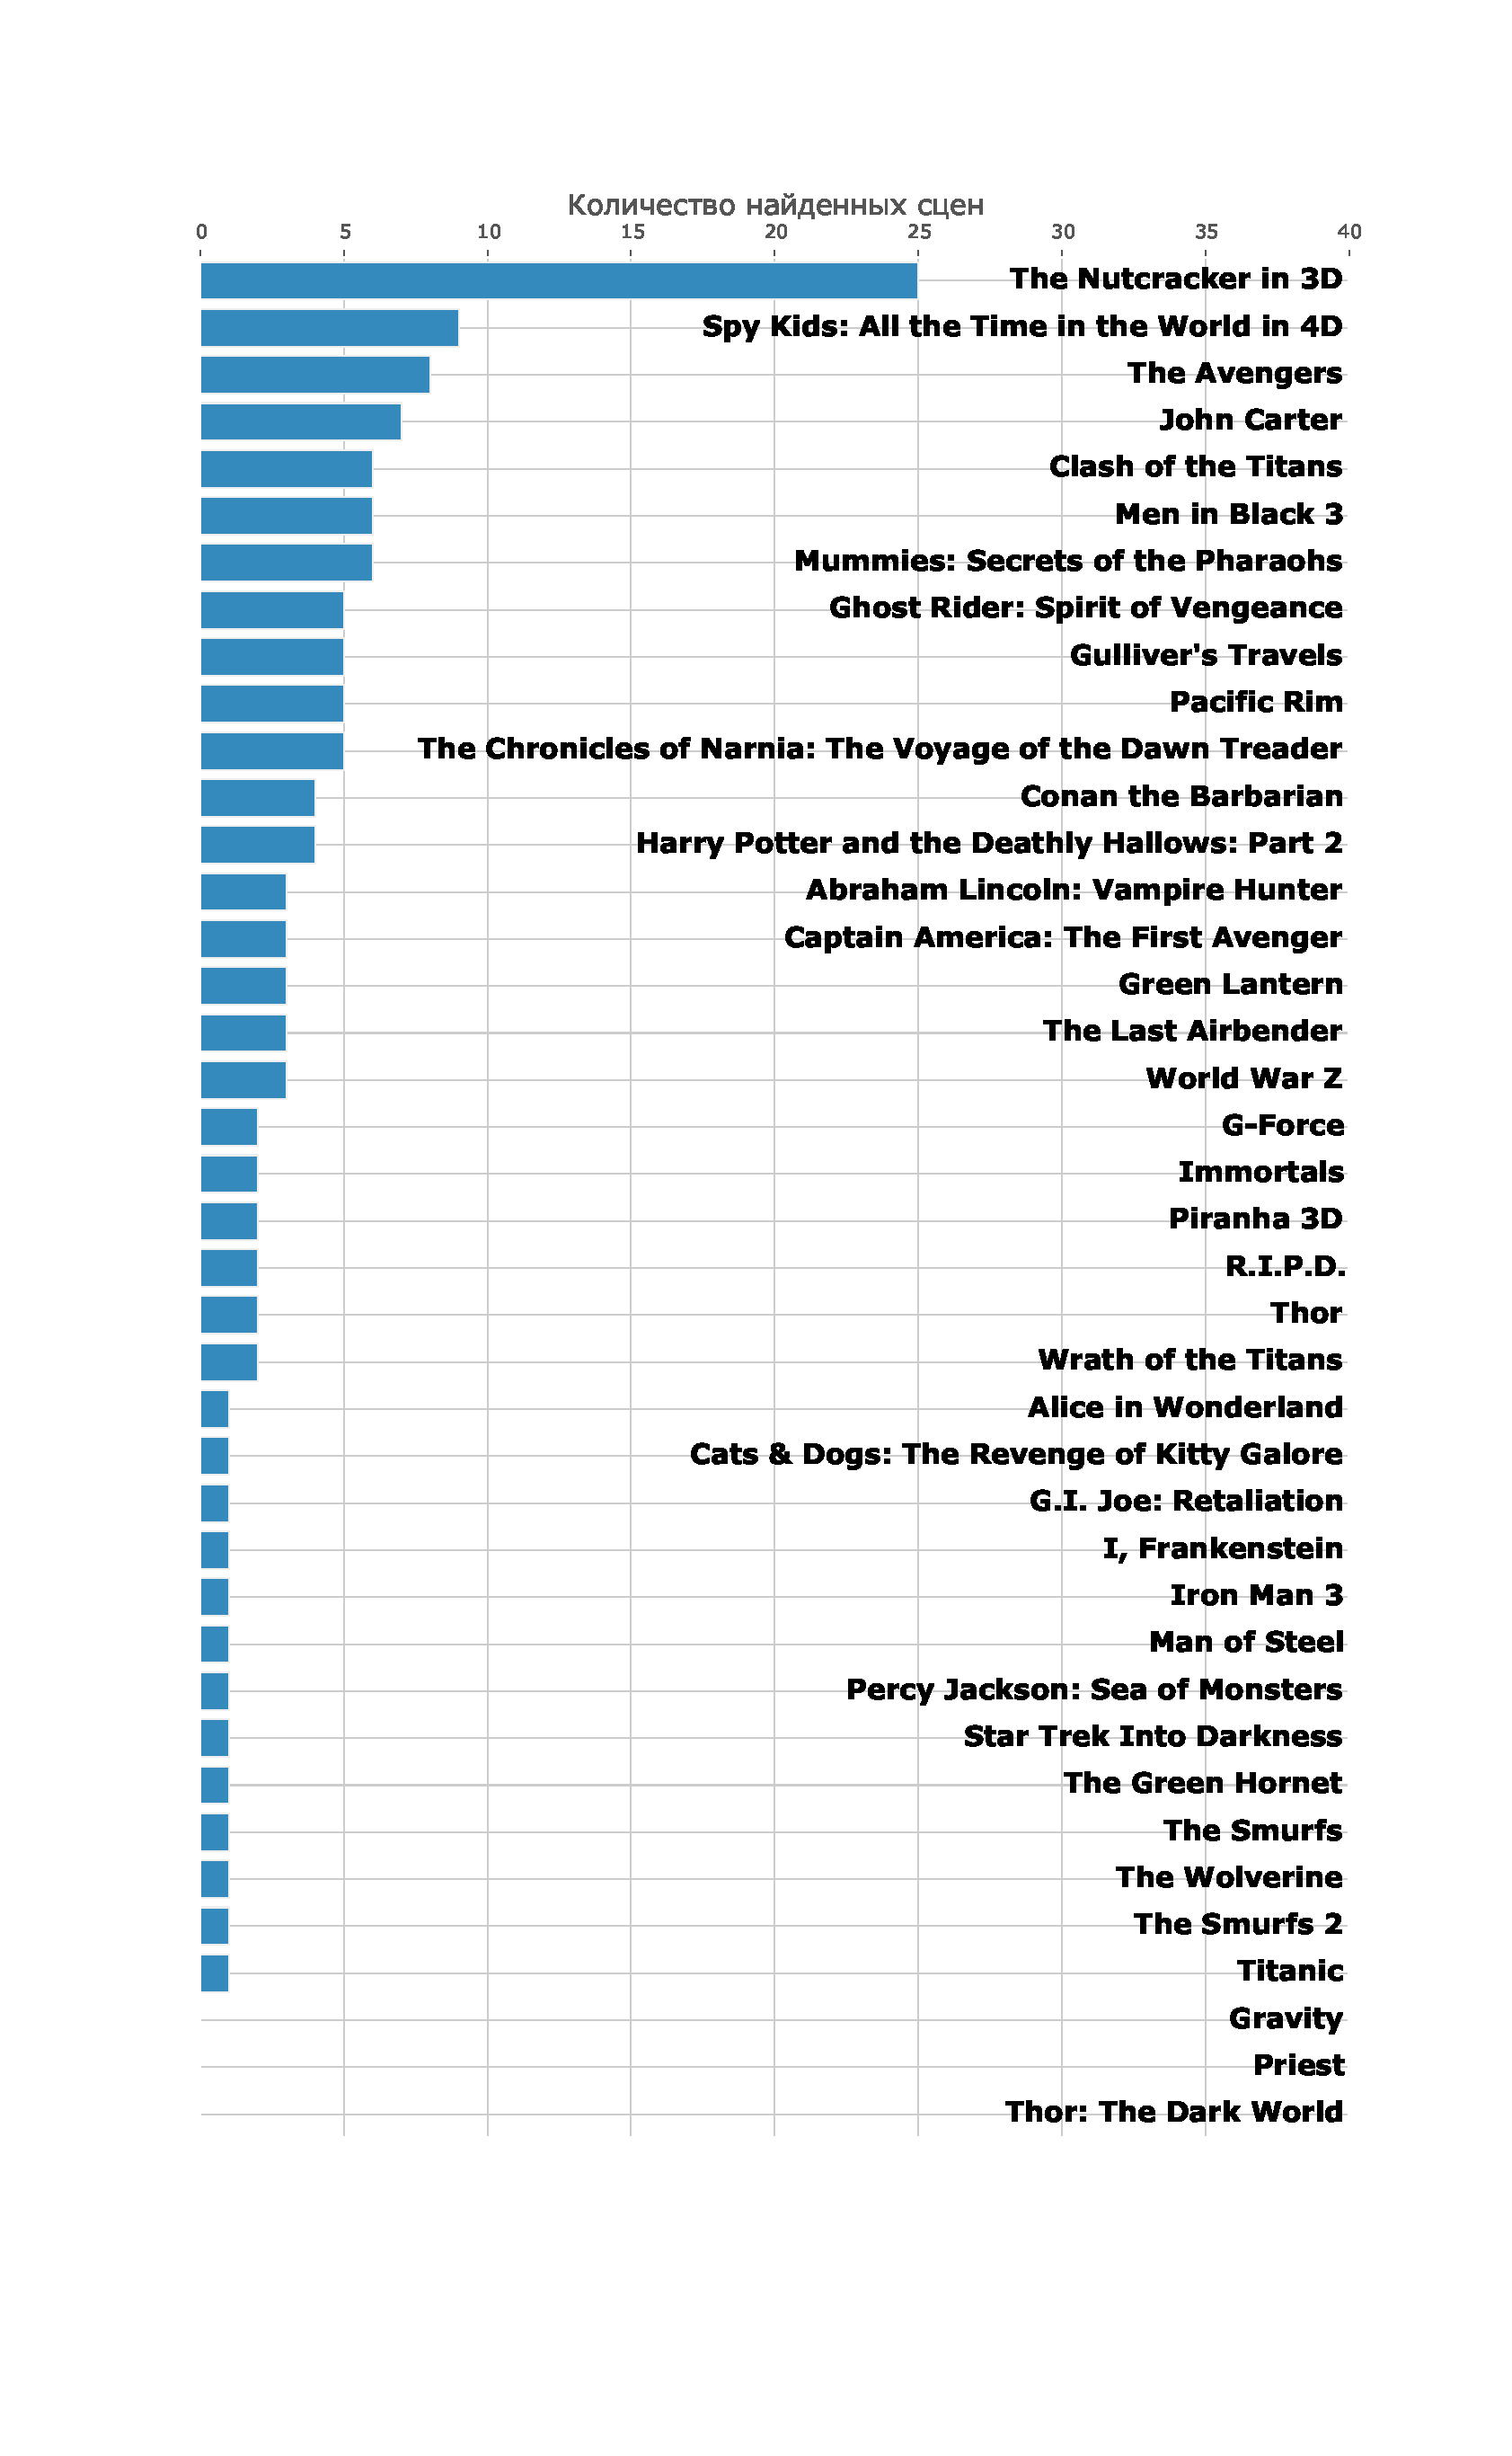
\includegraphics[width=0.82\textwidth, trim= 50 150 50 60, clip]{all_films_rus} }
	\end{minipage}
    \caption{Количество сцен с заметными артифактами, найденных 
    	в процессе анализа полнометражных фильмов.}
	\label{fig:results}
\end{figure}


The most common source of false-positive alerts were objects in front of textureless 
backgrounds (e.g., sky). Since the block-based disparity-estimation method fails 
to reliably estimate disparity for textureless areas, the proposed pipeline is unable to detect 
differences in object and background disparity even if the object appears in the depth map. 
Moreover, the human visual system is quite tolerant of missing depth differences in areas 
that lack color texture. Thus, the reasonable approach to decreasing the false-positive ratio
is to exclude from the algorithm's consideration any objects that appear in front of a uniform background.
We did so by weighting the output motion-edge map with the RGB variances of the input 
frame. Fig.~\ref{fig:textureless} shows  a comparison of  scores computed using the original 
and modified algorithms for scenes from the validation data set. The modified
algorithm manages to distinguish scenes with artifacts from scenes mistakenly detected
by its unmodified version.

\begin{table}[!h]
	\centering
	\begin{tabular}[width=\textwidth]{lcc}
		\toprule
		Film 										&  True positive  & False positive  		 \\\toprule
		Clash of the Titans 			& 5 								 & 5 						   \\\midrule
		Conan the Barbarian 		& 4 								 & 12 						  \\\midrule
		Star Trek Into Darkness   & 1 								    & 7 						  \\\midrule
		Harry Potter and  				&  									   &  							   \\
		the Deathly Hallows: 		 & 4 								   & 7						     \\
		Part 2 									  & 									  & 							 \\\midrule
		The Avengers 					 & 7 									& 0 						 \\\bottomrule
	\end{tabular}
    \caption{Number of true- and false-positive detections by initial algorithm for the validation data set.}
	\label{tab:testsample}
\end{table}


After modifying the algorithm we applied it to 39 S3D converted movies. In total,
the algorithm detected 125 problem scenes. Fig.~\ref{fig:results} depicts the per-film distribution.

The average run time of the proposed pipeline when processing a $960\times540$ frame size is 
3.5~seconds on a 2.67 GHz Intel Core i7 processor with 24 GB of RAM.

\begin{figure}[!h]
	\begin{minipage}[b]{1.0\linewidth}
		\centering
		\centerline{ 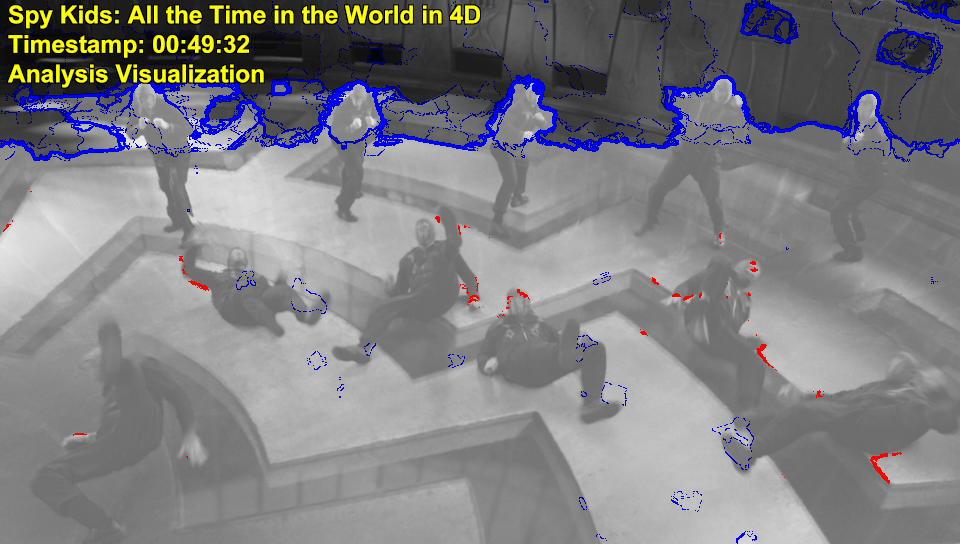
\includegraphics[width=0.8\textwidth]{example_spy} }
	\end{minipage}
	\begin{minipage}[b]{1.0\linewidth}
		\centering
		\centerline{ 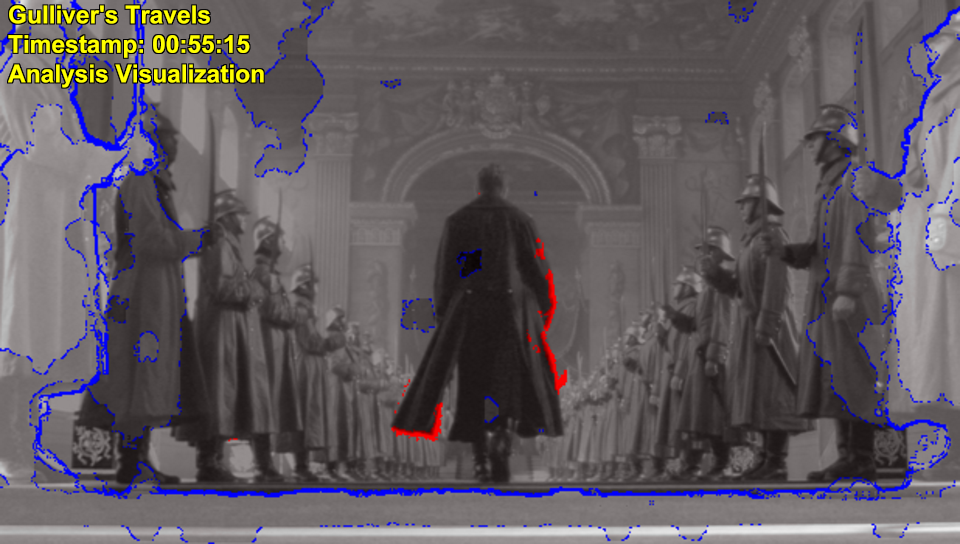
\includegraphics[width=0.8\textwidth]{example_gulliver} }
	\end{minipage}
    \caption{Пример результатов срабатвания алгоритма. В данных сценах
    	объекты переднего плана <<слиты>> с фоном. Для наглядности
    	поверх исходного кадра изображены карта диспаратности, границы
    	карты диспаратности (синие), и границы объектов, которые алгоритм посчитал
    	потерянными (красные).}
	\label{fig:res_example}
\end{figure}


\newpage
\section{Программная реализация}

\newpage
\section{Заключение}

\subsection{Результаты работы}

In this paper we proposed a method for assessing the quality of converted stereoscopic video.
The method detects foreground objects that are stuck to the background in the depth map and allows
filmmakers to correct the problem.

We demonstrated the performance of our method using a data set containing 
scenes from five S3D movies. We reduced the false-positive ratio by forcing it 
to ignore regions of uniform color. Use of fast depth-from-motion extraction enabled 
us to analyze 39 full-length converted S3D films and detect 125 scenes with significant 
artifacts that could cause visual discomfort.

\subsection{Направления для дальнейшего исследования}

\subsection{Публикации и гранты}

По теме данной работы были сделаны следующие публикации:

\begin{itemize}
	\item Dolganov S. et al. Detection of stuck-to-background objects in converted S3D movies // 3D Imaging (IC3D), 2015 International Conference on. – IEEE, 2015. – С. 1-6.
	\item Долганов С. В. <<Метод поиска несоответствий границ объектов между результатом 2D-3D конвертации и используемыми картами глубины>> // XXIII Международная конференция студентов, аспирантов и молодых ученых <<Ломоносов-2016>>, стр. 11-13.
\end{itemize}

Также работа была частично поддержана грантом РФФИ № 15-01-08632-а.

\newpage
\section{Приложения}

\newpage
%\section*{Список литературы}
\addcontentsline{toc}{section}{Список литературы}
\bibliographystyle{gost2008}
\bibliography{dipbib}

\end{document} 